\documentclass[main]{subfiles}


\title[AutoML: NAS]{Neural Architecture Search}
\subtitle{One-Shot Techniques in NAS}
\author[Jovita Lukasik]{Jovita Lukasik}
\date{}

\titlebackground*{images/AutoML_HPO_2_2}

%\institute{}
%\date{}

\begin{document}
	
	\maketitle


\begin{frame}{One-Shot Techniques in Neural Architecture Search}
\begin{center}
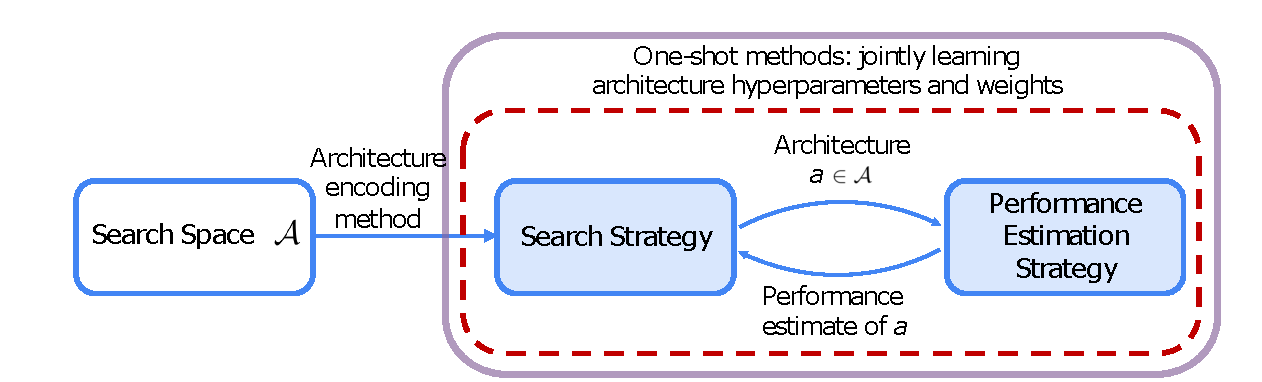
\includegraphics[height=3cm]{images/05/white_2023_nas_overview_4.pdf}
\captionof{figure}{Overview of neural architecture search ~\liturl{White et al. 2023}{https://arxiv.org/pdf/2301.08727.pdf}}
\end{center}
\end{frame}

\begin{frame}{Weight-Sharing and One-Shot Techniques}
The one-shot model can be seen as a directed acyclic multigraph
    \begin{itemize}
        \item Nodes: latent representations
        \item Edges: operations 
        \item Architecture optimization problem: Find optimal path from input to output
    \end{itemize}
\begin{center}
    
\includegraphics[height=2cm]{images/05/supernet_illustration.pdf}
    \captionof{figure}{Supernet illustration  ~\liturl{White et al. 2023}{https://arxiv.org/pdf/2301.08727.pdf}}
\end{center}
    
\end{frame}

\begin{frame}{Weight-Sharing and One-Shot Techniques}
\begin{itemize}
    \item Once one-shot model trained inherit weight for subnet from supernet 
    \item scalability and efficiency:
    \begin{itemize}
        \item Linear increase in number of candidates causes linear increase in computational costs for training but number of subnets increases exponentially 
    \end{itemize}
$\rightsquigarrow$ supernet allows to train exponential number of architectures in linear compute costs
\end{itemize}

\alert{Key assumption}: Ranking of architectures evaluated using one-shot model is relatively consistent with ranking one would obtain from training them independently	

Supernet allows quick evaluation, but still need to decide for search strategy (during supernet training or after)
\end{frame}

\begin{frame}{Weight-Sharing and One-Shot Techniques}
\begin{itemize}
    \item All possible architectures are subgraphs of a large subergraphs (one-shot model)
    \item Weights are shared between architectures
    \item Search costs are reduced since only training a single model

\end{itemize}
\end{frame}

\begin{frame}{DARTS}
    
\end{frame}
%----------------------------------------------------------------------
\begin{frame}{Summary} 

Most important insights from this video:

\begin{enumerate}
    \item ???
    \item ???
    \item ???
\end{enumerate}


\end{frame}



\end{document}
